%----------------------------------------------------------------------------------------
%	CHAPTER 4: Ripa Blockchain
%----------------------------------------------------------------------------------------

\chapterimage{chapter_head_4_Dubai.jpg} % Chapter heading image
\chapter{La Blockchain Ripa}
\label{sec:theRipaBlockchain}
Il progetto RipaEx avrà la propria blockchain che sarà denominata Ripa, securizzata tramite il protocollo DPOS e
con il proprio token XPX (simbolo \PHP) scambiato su di essa che servirà a svolgere le seguenti funzioni:
	\begin{enumerate}
		\item per listare nuove valute nell'exchange
		\item per pubblicizzare nuovi progetti
		\item per comprare gadget RipaEx nello Store RipaEx Store
		\item per pagare per l'acquisto di beni e servizi in rivenditori autorizzati tramite il RipaEx POV (Punto di Vendita)
		\item per condividere liquidità tra tutti gli exchnage della rete Ripa
	\end{enumerate}

Il token XPX è una criptovaluta derivata da ARK, Lisk, Crypti e BitShares con differenze uniche e miglioramenti per 
raggiungere l'obbiettivo di condividere liquidità tra tutti gli exchange della rete Ripa. Tuttavia questo codice eredita
le transazioni semplificate tra le blockchain basate su ARK ed il protocollo di consenso DPOS. Questo codice sorgente omogeneo 
permette lo sviluppo di potenziali servizi inter-blockchain nella forma di app ARK ed assieme ad altri sistemi addizionali
forniti dagli amministratori delle blockchain rispettive.

\vspace{5mm}
\textsc{\textbf{La blockchain Ripa è un fork di ARK e la creazione di tale blockchain serve per completare l'ecosistema Ripa
permettendo ogni exchange nella rete Ripa di condividere la stessa liquidità. Noi ci affideremo sempre ad ARK come nostro
fornitore di tecnologia blockchain di fiducia per includere il loro codice nei nostri repositori
per tutto ciò che riguarda la blockchain Ripa}}

\vspace{5mm}

Spiegato l'uso della blockchain Ripa all'interno dell'ecosistema RipaEx e spiegato il legame di partnership tecnologica
RIPA - ARK nelle seguenti sezioni potete trovare le specifiche della blokchain Ripa che sono derivata da ARK ed alcune sviluppate 
``ad hoc'' per l'ecosistema Ripa.

\section{Tecnologia Delegated Proof of Stake}
Ripa Blockchain eredita il sistema di consenso Delegated Proof of Stake (DPoS) che è stato inizialmente
introdotto da BitShares. Questo algoritmo di consenso è stato progettato per eliminare i problemi dell'algoritmo
Proof of Work (PoW), nello specifico la centralizzazione del potere computazionale e l'esponenziale uso di energia
elettrica. Anche se non completamente decentralizzato in quanto si basa su di un numero fisso di delegati eletti
dalla comunità, il DPoS garantisce migliore decentralizzazione di Bitcoin. L'algoritmo di consenso è migliorato
con il tempo, evolvendo in una procedura di consenso ottimale con il tempo.\\

Le specifiche tecniche di Ripa Blockchain sono le seguenti:
\begin{enumerate}
	\item DPoS (Delegated Proof of Stake)
	\begin{itemize}
		\item 101 delegati forgiani
		\item Delegati selezionati mediate un meccanismo di voto insito nel sistema DPoS
		\item 115,000,000 XPX - Forgiati nel Genesis Block
	\end{itemize}
	\item Account Multi-firma
	\item Reward di Blocco Costante
	\begin{itemize}
		\item 2 \PHP per blocco
		\item Livello di Inflazione (con blocco da 8s)
		\begin{itemize}
			\item 6.31\% per il primo anno
			\item 5.93\% il secondo anno
			\item 4.02\% il decimo anno
		\end{itemize}
		\item Tempo di forgiatura blocco di 8 secondi
		\begin{itemize}
			\item Tempo di forgiatura blocco riducibile nel tempo con aggiornamenti futuri del core.
		\end{itemize}
		\item 25 transazioni per blocco
		\begin{itemize}
			\item Incrementabile con soft fork se richiesto.
		\end{itemize}
	\end{itemize}
	\item Tabelle di routing
	\item Campo SmartBridge per uso con blockchain connesse alla blockchain RIPA principale (ARK Contract Execution Service)
	\item Transazioni batch\footnote{Aggiornamento futuro: quando ARK 2.0 sarà rilasciata \label{note1}}
	\item Fee di transazione personalizzabili\footnotemark[\value{footnote}]
	\item SmartContract nativi\footnote{Aggiornamento futuro: quando ARK Virtual Machine sarà rilasciata}
\end{enumerate}

\vspace{5mm}
\textsc{\textbf{Come detto Ripa Blockchain è un fork di ARK e noi ci affideremo sempre ad ARK come nostro provider di tecnologia 
di fiducia per includere il loro codice nelle nostre ultime funzionalità per tutto ciò che concerne lo sviluppo di 
Ripa Blockchain}}, funzionalità quali:
\begin{itemize}
	\item \textbf{Scalabilità della rete} al livello delle reti di Carte di Credito più diffuse con aggiornamento del core
	\begin{itemize}
		\item Aumentare il numero dei delegati forgianti
		\item Aumentare le dimensioni del blocco per includere più transazioni
		\item Implementazione del concetto di blocchi pre-approvati PBFT in testnet [nome in codice: TwinChain]
		\item Tabelle di routing per minimizzare i salti tra i nodi quando i blocchi sono trasmessi
		\item Inclusione di forgiato con nipoti RIPA
	\end{itemize}
	\item \textbf{Due tipi di nodi} sono usati per sicurizzare la rete RIPA:
	\begin{itemize}
		\item \textbf{Nodi di trasmissione} - Nodi con funzionalità di API che servono come back-end per servizi terzi
		(es: lite client). I nodi di trasmissione non forgiano blocchi e non quadagnano XPX per le transazioni.
		\item \textbf{Nodi forgianti} - Nodi con funzionalità API ridotta per abbassare l'esposizione a potenziali
		attacchi DDoS alla piattaforma RIPA. I nodi forgianti forgiano XPX e ricevono commissioni di transazione.
	\end{itemize}
	\item \textbf{Lite client ufficiale} per l'accesso al network è forinito poco dopo il lancio della mainnet ed 
	include il client desktop (Windows, MacOS e Linux) ed il client mobile (Android ed iOS)
	\item \textbf{Creazione offline di indirizzi}: la rete di per se non ha una Interfaccia Grafica Utente di 
	default, ogni account RIPA può essere creato off-line e gestito a costo zero su di un singolo dispositivo
	(computer, smartphone, tablet, ARM, IoT).
\end{itemize}

\section{Hierarchical Deterministic (HD) Wallets (BIP32)}
La struttura della chiave pubblica e privata di RIPA segue le stesse specifiche di Bitcoin. Una implementazione
personalizzata del protocollo BIP32 per Wallet Hierarchical Deterministic è fornita agli utenti RIPA.

\section{Commissioni}
Le commissioni per una transazione standard sono \PHP0,10 ma saranno flessibili in futuri rilasci di Ripa Blockchain.
Al lancio della mainnet, la struttura delle commissioni è fornita preconfigurata e pronta all'uso ai delegati
forgianti secondo le seguenti regole:
	\begin{itemize}
		\item Transazione \PHP0.1
		\item Voto \PHP1 (101 voti per transazione)
		\item Seconda Firma \PHP1
		\item Multi Firma \PHP1 per firma + \PHP1 per account firmatario
		\item Registrazione di un delegato \PHP25.
	\end{itemize}
Tutte le commissioni sono pagate ai nodi forgianti che processano i blocchi contenenti quelle commissioni.

\section{Delegati Ripa e Votazione}
Ogni nodo che esegue il codice della blockchain Ripa che vuole forgiare blocchi deve registrarsi come 
delegato pagando la commissione di 25 \PHP. Ripa incorpora un nuovo sistema di voto DPoS
originariamente progettato dai fondatori di Crypti. La commissione di voto è di 1 \PHP, 
il peso di voto di ciascun wallet è suddiviso equamente tra tutti i delegati votati 
nella transazione. Ad esempio: 
\begin{itemize}
	\item Se un wallet vota per un delegato, il delegato riceve il 100\% del peso di voto del
	wallet.
	\item Se il wallet vota per un delegato addizionale, il peso di voto totale è 
	suddiviso equamente tra entrambi i delegati al 50\%.
	\item Aggiungendo un terzo delegato, il peso di voto è suddiviso nuovamente, 
	ed ogniuno dei tre delegati riceve il 33,333\% del peso di voto del wallet.
\end{itemize}

I 101 delegati forgianti con il numero di voti maggiore sono elegibili per forgiare blocchi
RIPA. Questa progettazione elimina la possibilità che un singolo grande possessore di
RIPA oppure un'organizzazione che detiene una larga percentuale di RIPA siano in grado
di prendere il controllo della rete nella sua interezza mediante il voto dei loro nodi
ponendoli in posizione di nodi forgianti, prendendo, effettivamente controllo dell'intera rete. 
I voti provenienti dai token RIPA in possesso del Ripa Founder Team
possono essere usati a sola discrezione del team Ripa.

\section{Collegamenti tra Blockchain}
\subsection{Blockchain Connesse ARK (Tecnologia SmartBridge)}
La piattaforma ARK 1.0 non fornisce supporto diretto per sidechain o dapp. Invece
un meccanismo per connettere direttamente blockchain tra loro e con la blockchain ARK
è fornito tramite una funzione ponte codificata direttamente nel core ARK in cui
ogni blockchain può inviare e ricevere funzioni attivabili a comando e dati
informativi passando per la rete ARK principale tramite \textbf{Endoded Listeners}
e \textbf{SmartBridge} appositamente sviluppati.
\begin{center}
	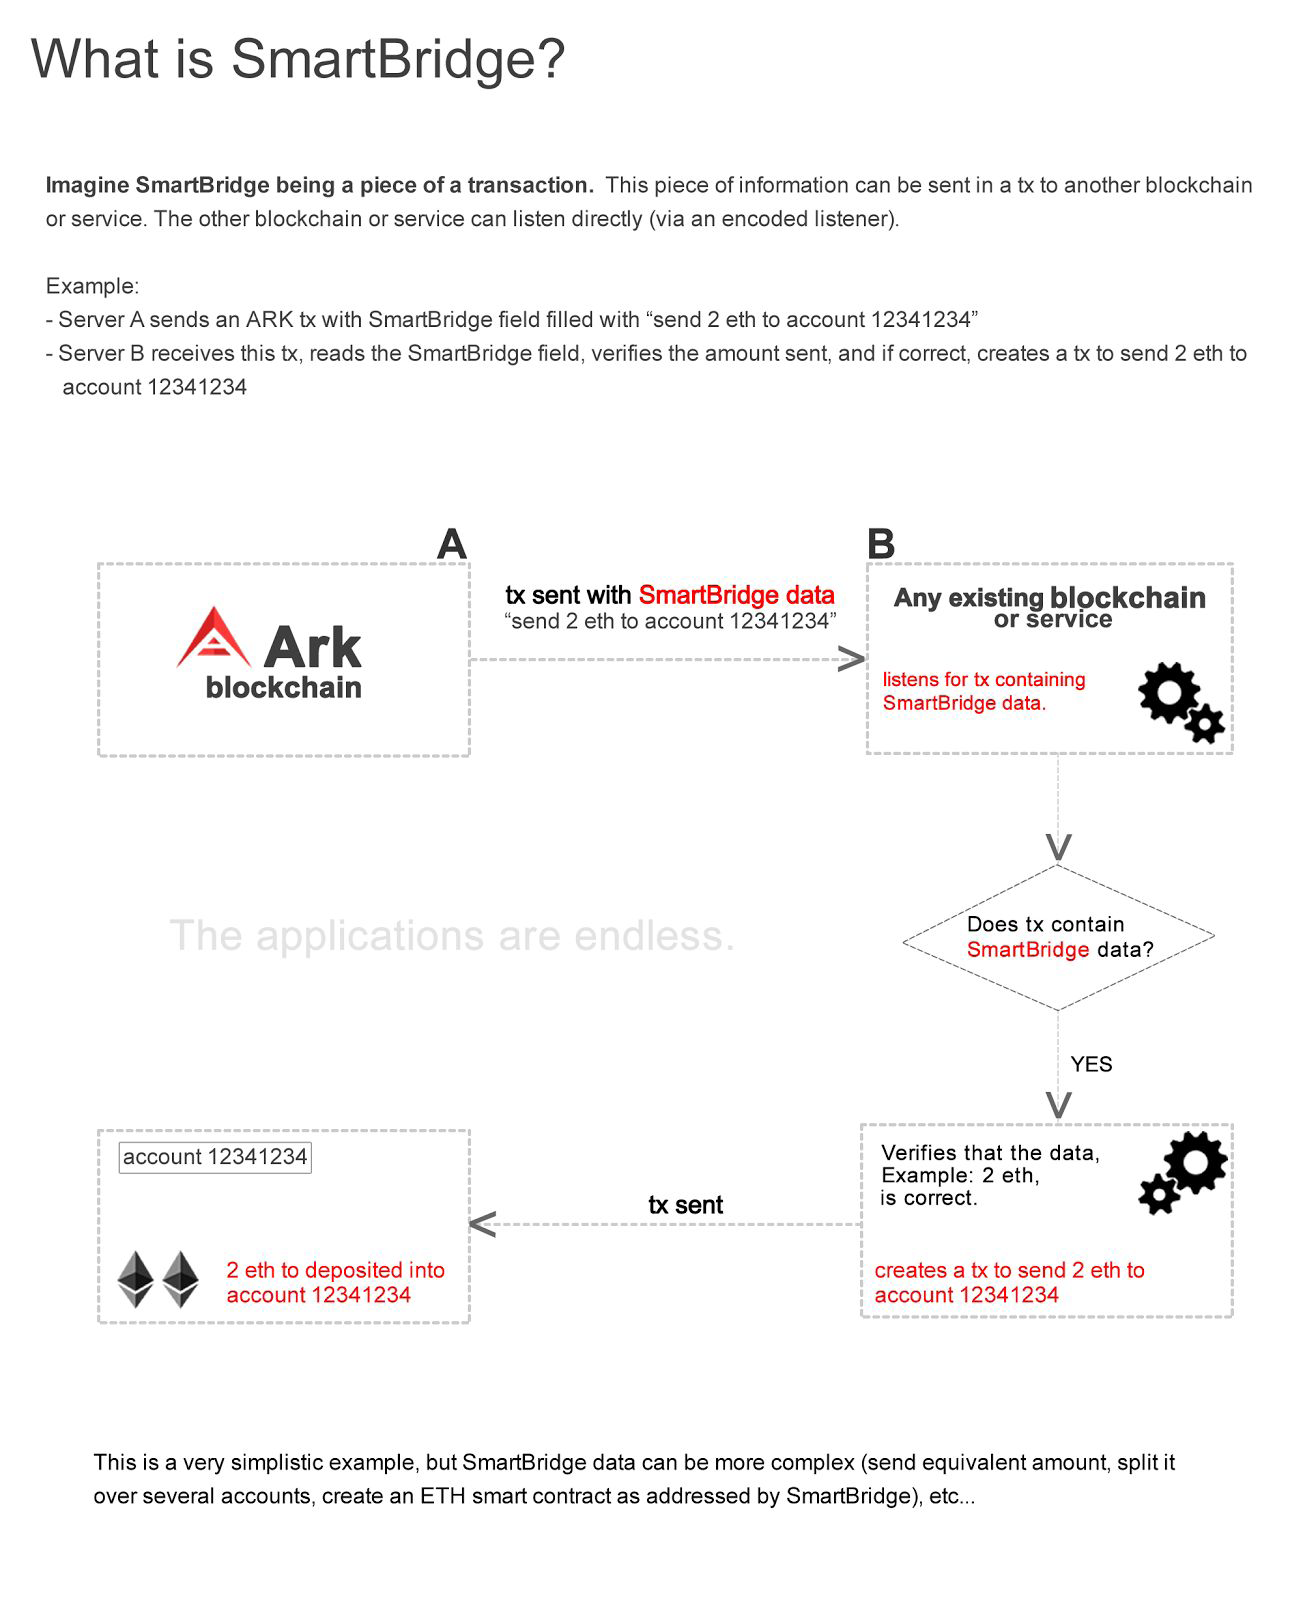
\includegraphics[width=\textwidth,height=\textheight,keepaspectratio]{ARKSmartBridge}
	\captionof{figure}{ARK Tecnologia SmartBridge}
\end{center}

\subsection{A.C.E.S. - ARK Contract Execution Service}
ACES è una piattaforma di interoperabilità tra blockchain che fornisce protocolli semplificati
e strumenti per costruire mercati di scambio servizi tra blockchain robusti.

ACES è composta principalmente dai tre componenti seguenti:
\begin{itemize}
	\item \textbf{Listener} i Listener ACES forniscono una via per tutti gli eventi delle diverse
	blockchain per essere facilmente consumanti via servizi REST. Le API permettono agli utenti
	di creare sottoscrizioni e ricevere eventi blockchain in tempo-reale usando callback Webhook.
	\item \textbf{Servizi} ACES che creano ed eseguono Service Contract, che possono essere qualsiasi
	cosa da caricare un file in una blockchain di dati, ad eseguire trasmissione di valore,
	creare smart contract, eseguire codice su di una piattaforma di computer distribuita, oppure
	interagire con dispositivi IoT.
	\item \textbf{Console di Mercato} di ACES è una dashboard utente per cercare ed eseguire Service
	Contract listati nel marketplace. I provider ACES possono listare i servizi dei loro nodi 
	usando le API del marketplace.
\end{itemize}

\begin{center}
	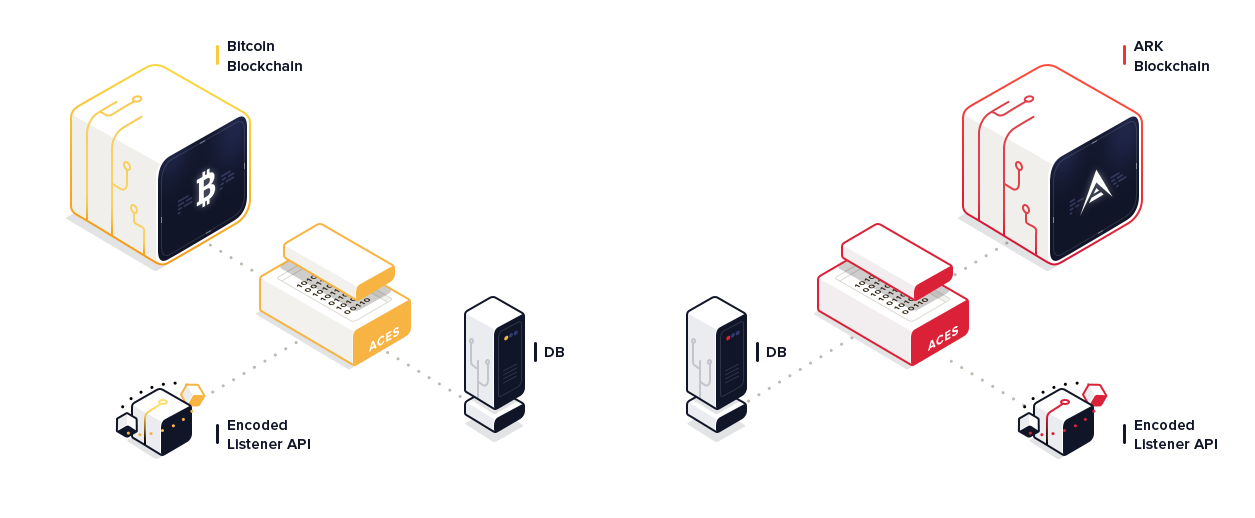
\includegraphics[width=\textwidth,height=\textheight,keepaspectratio]{ACES}
	\captionof{figure}{Implementazione SmartBridge ARK-BTC di A.C.E.S.}
\end{center}

\section{Ripa Liquidity Service Provider (R.L.S.P)}
Usando la tecnologia SmartBridge RipaEx svilupperà un meccanismo per condividere liquidità tra tutti gli exchange della rete
Ripa scrivendo i singoli orderbook in Ripa Blockchain ed eseguendo accoppiamento di ordini tra tutti gli exchange della rete.

In questo modo puoi avere i benefici di un exchange decentralizzato (come ad esempio la liquidità) con i benefici di un 
exchange centralizzato (come ad esempio customer support di livello platino e scambio FIAT).

\section{Ripa Community Fund}
Per permettere la nascita di nuovi exchange nella rete Ripa viene creato all'avvio del progetto il Fondo Comunitario Ripa - RCF - 
con le seguenti caratteristiche:
\begin{itemize}
	\item \textbf{Fondi di Partenza}: l'RCF avrà un capitale iniziale operativo pari al 5\% (5.750.000 \PHP) del blocco genesis
	\item \textbf{Fondi Ricorrenti}: ogni delegato contribuirà all'RCF con il 5\% degli XPX forgiati settimanalmente
\end{itemize}
\vspace{5mm}
Per ottenere i fondi dell'RCF per avviare il tuo Ripa Exchange devi inoltrare il tuo proposal nel sito ufficiale dell'RCF oppure
nella sezione RCF del forum Ripa in qualsiasi momento dopo l'avvio della prima istanza funzionante di Ripa Exchange.

